En esta sección, se busca resolver el problema de CMF a partir de una Heurística de Búsqueda Tabú (Tabu search\footnote{Glover, F. "Tabu Search — Part I", ORSA Journal on Computing 1989}). Dicha heurística consiste en una estrategia para resolver problemas combinatorios, aplicable tanto en grafos como en otras estructuras utilizadas para resolver problemas de lógica. Este método utiliza el mismo procedimiento que Búsqueda Local\footnote{Ver sección anterior.} para acercarse progresivamente a una mejor solución dentro de un entorno. Dado que en ciertos casos la solución no puede ser mejorada, la técnica de Búsqueda Tabú permite empeorarla parcialmente para proseguir la búsqueda de una mejor. A su vez, esta heurística concede una estructura llamada $lista\ tabú$ con distintas utilidades. Principalmente, sirve para guardar movimientos de modo a no repetirlos y/o guardar características o soluciones, entre otras. A continuación, se encuentra explicitado el pseudocódigo\footnote{http://www.dc.uba.ar/materias/aed3/2013/2c/laboratorio/heuristicas.pdf} de la heurística de Búsqueda Tabú:

\begin{algorithm}[H]
\SetAlgoLined
s$_{0}$ $\leftarrow$ solucion inicial \\
s$^{*}$ $\leftarrow$ s$_{0}$ \\
T $\leftarrow$ lista tabú inicial \\
\While{ no se alcance el criterio de terminacion}{
N $\leftarrow$ vecinos de s no tabú o mejores que s$^{*}$ \\
s $\leftarrow$ mejor solucion en N. \\
\If{ s es mejor que s$^{*}$}
 {s$^{*}$ $\leftarrow$ s} 
Actualizar la lista tabú T }
\end{algorithm}

\subsection{Explicación del algoritmo realizado}

 El algoritmo realizado parte de un valor entero positivo ingresado como parámetro, $desviacion\_permitida$, y de una solución provista por la Heurística de Búsqueda Local. A partir de esta última, el algoritmo busca, paulatinamente, una mejor solución siguiendo las siguientes opciones:
\begin{itemize}
 \item Agregando un nodo: Dada la solución actual (una clique), procede a $agregar$ un nodo que la mejore, es decir, que aumente su frontera.
 \item Quitando un nodo: Dada la solución actual (una clique), procede a $quitar$ un nodo que la mejore, es decir, que aumente su frontera.
\end{itemize}
A diferencia de la Búsqueda Local, se buscan nuevas soluciones que no necesariamente mejoren la solución obtenida hasta el momento pero que sí lo hagan a largo plazo. Sin embargo, dentro de las formas de empeorar la solución, se toma aquella que empeora lo menos posible. A su vez, a medida que se agrega o quita un nodo, se lo inserta en la lista tabú. Esto se realiza sin olvidar que siempre que pueda subir lo va a hacer, entonces, si descendiendo se encuentra con que puede volver a ascender, lo va a hacer hasta volver a estar en un máximo local.\newline

\begin{figure}[H] %[h] Aqui [b] para button [t] para top
\begin{center}
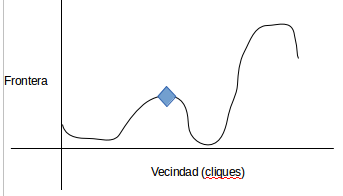
\includegraphics[width=250pt]{../imgs/1_tabu.png}
\caption{solución con Busqueda Local}
\subcaption{Aqui se muestra en el dominio la vecindad y en la imagen el valor de la frontera. El rombo rojo representa la solucion de la Busqueda Local.}
\end{center}
\end{figure}


\begin{figure}[H] %[h] Aqui [b] para button [t] para top
\begin{center}
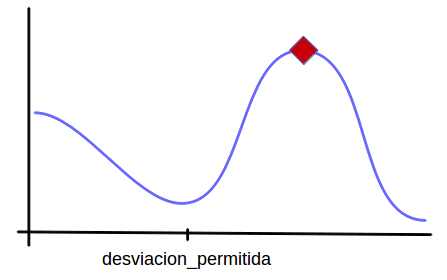
\includegraphics[width=250pt]{../imgs/2_tabu.png}
\caption{solución con Busqueda tabú}
\subcaption{Este es el mismo grafico anterior pero se puede notar como despues de aplicar $desviacion_permitida$ "descensos" la solucion comienza a mejorar hasta para en otro maximo local (mejor que el dado por Busqueda Local).}
\end{center}
\end{figure}

Al finalizar, el algoritmo retorna la mejor solución hallada. \newline

\textbf{Descripción de la lista tabú} \newline

 A medida que se van agregando o quitando nodos que no mejoran la solución, se los va marcando como tabú. De esta forma, se le asigna una prioridad a cada uno de ellos que depende del momento en que fue agregado. A su vez, sea cual sea la prioridad del último nodo insertado, éste no puede utilizarse en la iteración siguiente para evitar ciclar soluciones. Para lograr esto, hicimos que en el peor de los casos sólo se puedan usar los nodos tabús que tienen prioridad menor a la mitad de la prioridad máxima. Las ventajas de esto es que evitamos ciclar con los mismos nodos (por ejemplo, agregando y quitando un nodo) y a su vez permite trabajar con nodos de manera mas dispersa y no siempre con los mismos. Las desventajas es que cuando uno realiza una operación $p$ con un nodo $u$, y había otra operación $p'$ que aplicada al nodo $u$ producía menos frontera, se va a elegir realizar la operación $p$, pero por ahí para llegar a la optima había que realizar la operación $p'$ y esto no se va a realizar a corto plazo ya que el nodo es puesto como tabú.\newline

\textbf{Criterio de terminación} \newline

 El algoritmo presentado tiene dos criterios de terminación. Por un lado, la cantidad de iteraciones en que la solución puede mejorar y, por el otro, la variable $desviacion\_permitida$ ingresada como parámetro. El primero se encuentra acotado por el máximo absoluto que existe pues el problema siempre tiene solución. Luego, pueden existir muchos máximos locales pero ninguno será una clique con mayor frontera que la del máximo absoluto (esto resulta trivial). Por otro lado, la variable $desviacion\_permitida$ va disminuyendo cada vez que se modifica la solución actual sin mejorarla, es decir, que permitimos avanzar de manera ``no creciente'' una cantidad $desviacion\_permitida$ de veces. \newline




\begin{algorithm}[H]
    \SetAlgoLined
    \caption{TabuSearch}
    \KwIn{\textbf{Conj(nodos)} $solución\_inicial$, \textbf{Grafo} $g$, \textbf{Entero} $desviacion\_permitida$}
    \KwOut{\textbf{Conj(nodos)} $solución\_final$}

	\textbf{Conj(nodos)} sol$_{0}$,sol$_{1}$ \\ 
	\textbf{Conj(nodos)} $solución\_actual$ $\leftarrow$ LocalSearch($solución\_inicial$, $g$)	\\	
	\textbf{Conj(nodos)} $solución\_final$ $\leftarrow$ $solución\_actual$	\\	
	\textbf{Lista Tabu} $\leftarrow$ $\{\}$\\
	\textbf{Boolean} $Mejore\ la\ frontera$ $\leftarrow$ true

	\While{ $Mejore\ la\ frontera$ $\vee$ 0 $<$ $desviacion\_permitida$}{

	 	sol$_{0}$ $\leftarrow$ Dame Mejor solución agregando nodo No Tabu ($solución\_inicial$,$solución\_final$) \\
		sol$_{1}$ $\leftarrow$ Dame Mejor solución quitando nodo No Tabu ($solución\_inicial$,$solución\_final$) \\
		\If{ frontera(sol$_{0}$) $<$ frontera(sol$_{1}$)}
			{sol$_{0}$ $\leftarrow$ sol$_{1}$}
		\eIf{ frontera($solución\_actual$) $<$ frontera(sol$_{1}$)}
			{$solución\_actual$ $\leftarrow$ sol$_{0}$ \\
			$Mejore\ la\ frontera$ $\leftarrow$ true
			}
			{$Mejore\ la\ frontera$ $\leftarrow$ false \\
			 Poner Tabu Nodo utilizado en sol$_{0}$ \\
			 $desviacion\_permitida$ = $desviacion\_permitida$ - 1}
		$solución\_actual$ $\leftarrow$ sol$_{0}$ \\
		\If{ frontera($solución\_final$) $<$ frontera($solución\_actual$) } 
		{$solución\_final$ $\leftarrow$ $solución\_actual$}			
	}

    	\textbf{devolver} $solución\_final$ \\

\end{algorithm}

\begin{algorithm}[H]
    \SetAlgoLined
    \caption{Dame Mejor solución agregando nodo No Tabu}

	$solución\_final$ $\leftarrow$ $solución\_inicial$ con un nodo mas cualquiera \\
	\ForAll{$u \in Candidatos\_clique($solución\_inicial$)$}{
	 		\If{$u$ $\notin Nodos(solución\_inicial)$}{
				\eIf{$\neg$ es tabu($u$)}{
		 			\If{frontera($solución\_final$) $<$ frontera( $solución\_inicial$ con $u$) }{
						$solución\_final$ $\leftarrow$ $solución\_inicial$ con $u$}
				}{
					\If{ Es Tabu aceptable ($u$) $\land$ frontera($solución\_final$) $<$ frontera( $solución\_inicial$ con $u$)}
					{$solución\_final$ $\leftarrow$ $solución\_inicial$ con $u$}
				
				}
			}
	}

\end{algorithm}

\begin{algorithm}[H]
    \SetAlgoLined
    \caption{Dame Mejor solución quitando nodo No Tabu}

	$salida\_mejor$ $\leftarrow$ tomar primer nodo de $solución\_inicial$ \\
	$salida\_valor$ $\leftarrow$ grado del primer nodo \\
	\ForAll{$u \in$ Nodos($solución$\_$inicial$)}{
		\eIf{$\neg$ es tabu($u$)}{
	 		\If{ grado($u$) $<$ $salida\_valor$ }{
	 			$salida\_mejor$ $\leftarrow solución\_inicial$ sin $u$ \\
				$salida\_valor$ $\leftarrow grado\ nodo\ u$ }
		}{
				\If{Es Tabu aceptable ($u$) $\land$ grado($u$) $<$ $salida\_valor$}
				{
					$salida\_mejor$ $\leftarrow solución\_inicial$ sin $u$ \\
					$salida\_valor$ $\leftarrow grado\ nodo\ u$ \\
				}
		}
	}

\end{algorithm}

Donde:
\begin{itemize}
 \item $desviacion\_permitida$ consiste en la cantidad de veces que se agrega o quita un nodo por iteración (empeorando la solución parcial).
 \item $frontera$ es una función que, dada una clique pasada como parámetro, devuelve su frontera.
 \item $Candidatos\_clique$ devuelve los nodos que pertenecen a la clique máxima a partir de un conjunto de éstos pasado como parámetro.
 \item $Nodos$ devuelve los nodos pertenecientes a la solución pasada como parámetro.
 \item $Es\ tabú\ aceptable$ verifica si la prioridad de un nodo perteneciente a la lista tabú es menor a la mitad de la prioridad máxima, en cuyo caso se define como aceptable.
\end{itemize}

\subsection{Complejidad Temporal}

 A continuacion vamos a desarrollar la complejidad de este algoritmo a partir del pseudocodigo presentado anteriormente. \newline

 Cuando hablamos de una ``solución'' en el código, nos referimos a un vector que contiene los nodos pertenecientes a una clique. \newline

 Como puede observarse las operaciones como agregar o quitar un nodo consisten en realizar los siguientes pasos: \newline
\begin{itemize}
 \item $Copiar\ una\ solución$ actual a una nueva esto es lineal en la cantidad de nodos de la solucion.
 \item $Agregar\ un\ nodo$ consiste en calcular los candidatos a agregar en la solucion (tiene un coste de $\mathcal{O}(n)^{2}$ ya que recorre todos los nodos del grafo y por cada iteracion recorre todos los de la clique realizando comparaciones constantes) y una vez obtenido esos se recorren esos candidatos (lineal en cantidad de nodos) y se busca cual mejora la frontera (ver la frontera\footnote{Ver complejidad de estructura $Grafo$} de un nodo es $\mathcal{O}($cant.nodos$)$) de esta majera, encontrar el mejor es $\mathcal{O}($cant.nodos$)^{2}$. Luego, la complejidad final de esta operacion es $\mathcal{O}($cant.nodos$)^{2}$ + $\mathcal{O}($cant.nodos$)^{2}$ = $\mathcal{O}($cant.nodos$)^{2}$.
 \item $Quitar\ un\ nodo$ donde simplemente se busca el nodo con menor grado (esto es lineal en la cantidad de elementos y ver el grado es constante\footnote{Ver complejidad de estructura $Grafo$}), luego se crea una nueva solucion con los nodos anteriores menos el de menor grado (esto es lineal en $cant.nodos$). Luego, la complejidad de esta operacion es $\mathcal{O}($cant.nodos$)$) + $\mathcal{O}($cant.nodos$)$) = $\mathcal{O}($cant.nodos$)$).
\end{itemize}

 Por otro lado, la lista tabú esta representada por un vector de $n$ elementos donde en la i-esima posición esta el "valor tabú" del i-esimo nodo. Por lo tanto, poner como tabú a un nodo o ver su valor es equivalente a acceder\footnote{http://www.cplusplus.com/reference/vector/vector/operator[]/} a un elemento del arreglo que es constante.\newline

 Teniendo en cuenta todo lo anterior, notar que las operaciones $Dame$ $Mejor$ $solución$ $agregando$ $nodo$ $No$ $tabú$ y $Dame$ $Mejor$ $solución$ $agregando$ $nodo$ $No$ $tabú$ hacen referencia a $Agregar\ un\ nodo$ y $Quitar\ un\ nodo$ repectivamente.\newline

 Solo queda ver la complejidad de la función principal "TabuSearch". Esta comienza realizando una búsqueda local\footnote{ver sección anterior} (O(n$^{4}$)) la cual es almacenada en una solución (guardar dicha solución cuesta cuadrático en la cantidad de nodos); seguido define la lista tabú en 0 todos los valores (lineal en cantidad de nodos). Continuando empieza un ciclo ($desviacion_permitida$ + $cant.nodos$$^{2}$ en el peor caso) y por cada iteración se ejecuta las funciones $Dame$ $Mejor$ $solución$ $agregando$ $nodo$ $No$ $tabú$ y $Dame$ $Mejor$ $solución$ $agregando$ $nodo$ $No$ $tabú$ (O($cant.nodos$$^{2}$)+O($cant.nodos$)) seguido de comparaciones (lineal) y asignaciones con coste lineal. (Notar que las comparaciones son constantes pero ver la frontera es lineal). \newline
 De esta manera la complejidad final del algoritmo es $\mathcal{O}(n^{4})$ + $\mathcal{O}(n^{2})$ * $\mathcal{O}(n^{2})$ = $\mathcal{O}(n^{4})$.  \newline

Notar que la complejidad es similar a la de local porque, por un lado, se empieza realizando una búsqueda local (para tomar la solución inicial) y luego se realizan operaciones similares a las de dicha búsqueda (agregar y quitar nodos) por lo tanto tienen la misma complejidad y la cantidad de veces que se realizan es, al igual que la local,  una cantidad de iteraciones equivalente a los nodos al cuadrado mas una desviacion que es lineal en la cantidad de nodos.


\subsection{Instancias problemáticas}

 Aquí detallaremos instancias donde nuestra heuristica no encuentra soluciones cercanas a las optimas, o aun peor, se puede empeorar la solución cuanto uno quiera.

\begin{itemize}
 
  \item $La$ $solución$ $inicial$ $va$ $a$ $condicionar$ $la$ $final$. Como la solución inicial se encuentra en un máximo local solo le queda a la búsqueda "descender" en busca de un "nuevo ascenso" (Con ascender o descender nos referimos a mejorar o empeorar la solución actual respectivamente).


  \item $El$ $conjunto$ $de$ $cliques$ $sepadaras$ $por$ $n/2+1$ $afectan$ $la$ $solución$. Cuando tenemos varias cliques máximas separadas por dicha cantidad de aristas puente, nosotros empezamos a explorar en una (que es donde la búsqueda local termino), si la solución optima se encuentra en otra clique a la que los separa dicha cantidad de aristas, el algoritmo no va a poder llegar a encontrar dicha solucion. 

\end{itemize}

A continuación mostraremos un ejemplo en el que se dan ambos cosos y uno puede hacer tan mala como quiera la solucion.

 Al partir de un nodo con mayor grado, si la clique que tiene mayor frontera no posee a dicho nodo, hay muchas menos chances que el algoritmo encuentre la solución. De esta manera podemos definir la clase:
 $Grafo$ $con$ $una$ $estrella$ $y$ $una$ $clique$ $de$ $nodos$ $con$ $grado$ $menor$ $al$ $grado$ $central$ $de$ $la$ $estrella.$ 

\begin{figure}[H] %[h] Aqui [b] para button [t] para top
\begin{center}
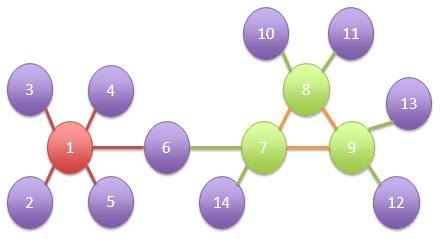
\includegraphics[width=250pt]{../imgs/ej1local.jpg}
\caption{Ejemplo Posible - Usado tambien en Local}
\end{center}
\end{figure}

\textbf{Formato de entrada:}

$$14\ \  14$$
$$1\ \  2$$
$$1\ \  3$$
$$1\ \  4$$
$$1\ \  5$$
$$1\ \  6$$
$$6\ \  7$$
$$7 \ \ 8$$
$$8\ \  9$$
$$9\ \  7$$
$$8\ \  10$$
$$8\ \  11$$
$$9\ \  12$$
$$9\ \  13$$
$$7\ \  14$$


\textbf{Formato de salida:}
$$5\ \   1\ \   1$$

\textbf{Solución Óptima:}
 $$6\ \   3\ \   7\ \   8\ \   9$$\newline

Se puede observar como a medida que uno agrega adyacentes a los nodos $7$, $8$ o $9$ tal que el nodo de mayor grado sea el $1$ la solucion va a ser tan mala como uno quiera, por ejemplo, agregandole mas adyacentes a $1$, para asi poder aumentar la cantidad de nodos de la frontera de la clique optima. \newline

Notar que la mayoría de problemas encontrados se deben al proceso de intensificación, aunque en muchos casos puede ser muy favorable, en otros seria mejor aplicar técnicas de diversificación, como por ejemplo, variar la entrada por nodos de diferentes cliques máximas, colaborando mucho en la búsqueda de soluciones mas diversas.

\subsection{Experimentación}

 En esta sección buscamos encontrar un numero correcto para asignarle $desviacion\_permitida$ de tal forma de amortiguar lo mas posible tiempo con resultados. \newline
 El siguiente gráfico muestra, para diferentes $desviacion\_permitida$ y una densidad de aristas igual al 50$\%$ respecto a los nodos, el resultado temporal, y luego de calidad. Los grafos son aleatorios, este tipo de grafos son explicitados mas adelante en la sección $Experimentacion\ General$.


\begin{figure}[H] %[h] Aqui [b] para button [t] para top
\begin{center}
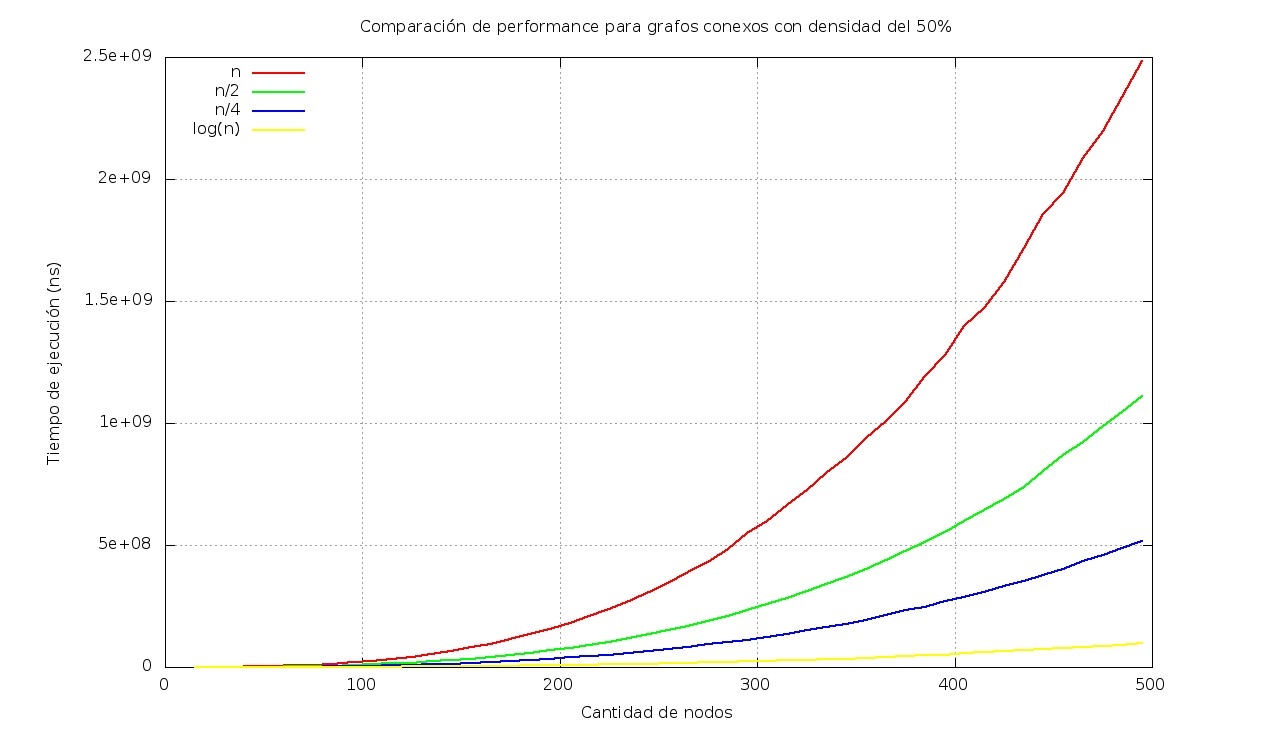
\includegraphics[width=400pt]{../imgs/variaciontemporal_tabu.jpg}
\caption{Variacion de $desviacion\_permitida$ - Grafico Temporal}
\end{center}
\end{figure}

\begin{figure}[H] %[h] Aqui [b] para button [t] para top
\begin{center}
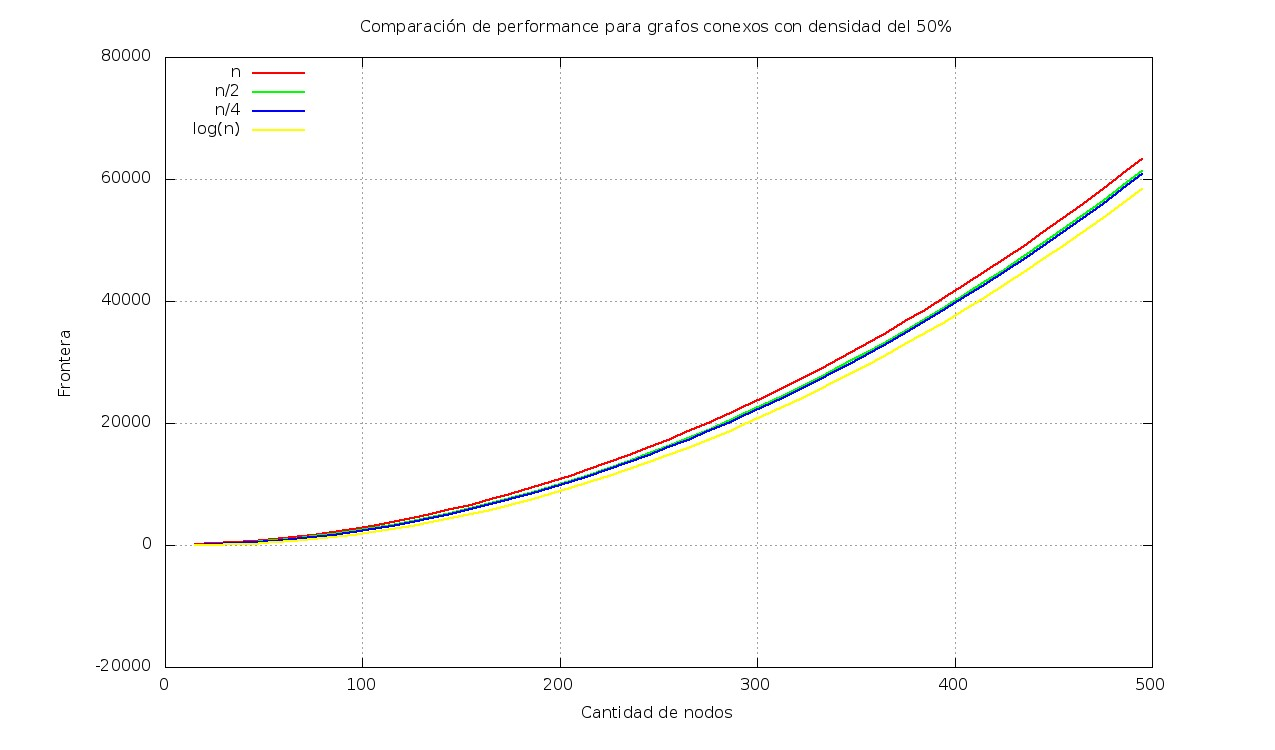
\includegraphics[width=400pt]{../imgs/variacioncalidad_tabu.jpg}
\caption{Variacion de $desviacion\_permitida$ - Grafico de Calidad}
\end{center}
\end{figure}

El siguiente gráfico muestra un promedio entre el tiempo que tarda y el resultado obtenido.

\begin{figure}[H] %[h] Aqui [b] para button [t] para top
\begin{center}
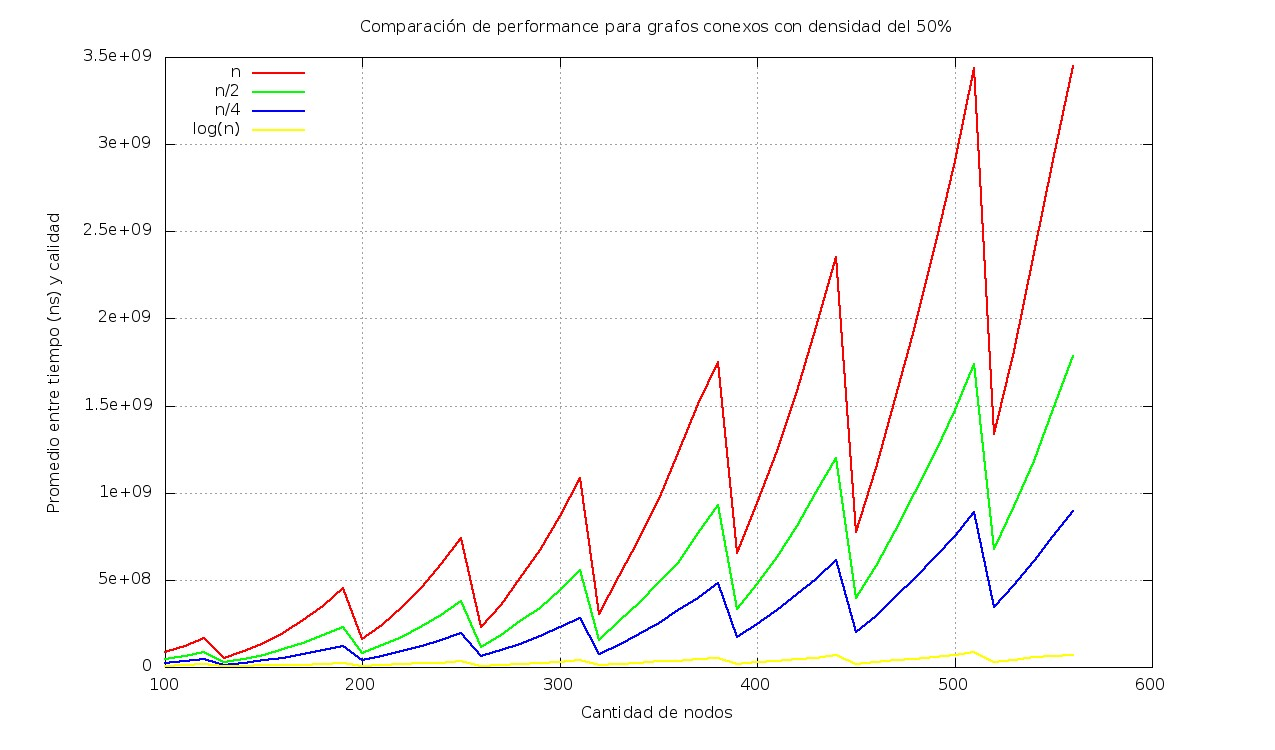
\includegraphics[width=400pt]{../imgs/variacionpromedio_tabu.jpg}
\caption{Variacion de $desviacion\_permitida$ - Grafico Promedio entre calidad y tiempo}
\end{center}
\end{figure}

 Cuando hablamos de promedio hacemos referencia a un balance entre tiempo y calidad. Elegimos esto ya que,  para realizar diferentes experimentaciones con los grafos, dado la densidad y la cantidad de pruebas que hacemos no nos es viable que tarde mucho en procesar cada grafo. A su vez, tampoco queremos que las soluciones nunca mejoren a la local, porque no tendría sentido. Es por esta razón que elegimos el promedio.

 De esta manera podemos observar que para una densidad de 50$\%$ de aristas un valor promedio optimo es $n/2$ con $n$ = $cantidad\ de\ nodos$. Es por esta razón que en los items anteriores usamos este valor. Elegimos este valor, aunque también pudimos haber elegido $n/4$, pero cuanto mas chico, en grafos con pocas aristas va a contemplar muchos menos casos.

